\documentclass{article}
\usepackage{pgfplots}
\pgfplotsset{compat=1.18}

\begin{document}

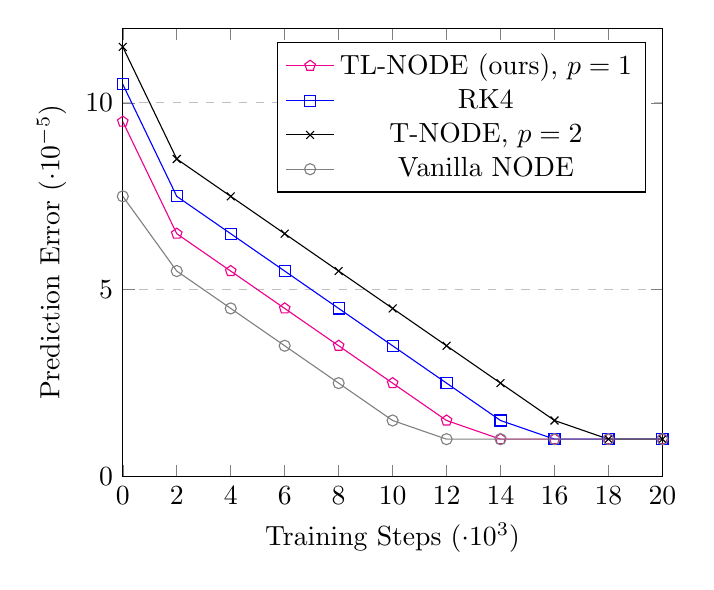
\begin{tikzpicture}
    \begin{axis}[
        xlabel={Training Steps ($\cdot 10^3$)},
        ylabel={Prediction Error ($\cdot 10^{-5}$)},
        xmin=0, xmax=20,
        ymin=0, ymax=12,
        xtick={0,2,...,20},
        ytick={0,5,...,12},
        legend pos=north east,
        ymajorgrids=true,
        grid style=dashed,
    ]
    
    % TL-NODE (ours), p = 1
    \addplot[
        color=magenta,
        mark=pentagon,
        ]
        coordinates {
            (0,9.5)
            (2,6.5)
            (4,5.5)
            (6,4.5)
            (8,3.5)
            (10,2.5)
            (12,1.5)
            (14,1.0)
            (16,1.0)
            (18,1.0)
            (20,1.0)
        };
        \addlegendentry{TL-NODE (ours), $p=1$}
        
    % RK4
    \addplot[
        color=blue,
        mark=square,
        ]
        coordinates {
            (0,10.5)
            (2,7.5)
            (4,6.5)
            (6,5.5)
            (8,4.5)
            (10,3.5)
            (12,2.5)
            (14,1.5)
            (16,1.0)
            (18,1.0)
            (20,1.0)
        };
        \addlegendentry{RK4}
        
    % T-NODE, p = 2
    \addplot[
        color=black,
        mark=x,
        ]
        coordinates {
            (0,11.5)
            (2,8.5)
            (4,7.5)
            (6,6.5)
            (8,5.5)
            (10,4.5)
            (12,3.5)
            (14,2.5)
            (16,1.5)
            (18,1.0)
            (20,1.0)
        };
        \addlegendentry{T-NODE, $p=2$}
        
    % Vanilla NODE
    \addplot[
        color=gray,
        mark=o,
        ]
        coordinates {
            (0,7.5)
            (2,5.5)
            (4,4.5)
            (6,3.5)
            (8,2.5)
            (10,1.5)
            (12,1.0)
            (14,1.0)
            (16,1.0)
            (18,1.0)
            (20,1.0)
        };
        \addlegendentry{Vanilla NODE}
        
    \end{axis}
\end{tikzpicture}

\end{document}